\chapter{الأجهزة الحسية}\label{ch:b3:sensory-systems}

في ليلة مظلمة تقدر عين الإنسان على كشف ومضة من بضعة فوتونات
--- وهي أصغر كمية من الضوء تسمح الفيزياء بكشفها أصلًا.
والأذن تسمع صوتًا يحرّك طبلتها بأقل من قطر ذرة هدروجين،
وتميّز نغمة من أخرى تختلف عنها بخُمس في المئة. والكلب يتبع
أثرًا من بضعة جزيئات في السنتيمتر المكعب؛ والقرش يجد سمكة
مفلطحة تحت الرمل بالحقل الكهربائي لنبض قلبها. فكل حاسة تبدأ
بخلية تحوّل ضربًا من الطاقة إلى تغيّر في كمون الغشاء، وكل
حاسة تنتهي شوكاتٍ في عصب؛ وبين الاثنين تقع المسائل التي
يتناولها هذا الفصل: كيف يضخّم مستقبِل جزيئًا واحدًا أو
فوتونًا واحدًا إلى إشارة يقدر عصبون على قراءتها، وكيف يُضغط
مدى يبلغ تريليون ضعف في الشدة إلى معدل من بضع مئات من
الشوكات في الثانية، وكيف تُفرز موجة ميكانيكية بحسب التردد،
وكيف تُميَّز عشرة آلاف رائحة بأربعمئة مستقبل، وكيف يعرف
الدماغ، الذي لا يصله إلا الشوكات، من أي حاسة جاءت.

\section{مبادئ مشتركة بين كل الحواس}

\begin{definition}[التحويل، والترميز، والتكيّف]\label{def:b3:sensory-systems:principles}
\index{تحويل حسي}\index{كمون المستقبِل}\index{خط موسوم}\index{حقل استقبالي}\index{تكيّف!حسي}\index{تثبيط جانبي}
تحوي \emph{الخلية المستقبِلة الحسية} آلية \emph{تحويل} ---
بروتينًا أو شلالًا --- تحوّل منبّهًا (فوتونًا، أو جزيئًا، أو
إزاحة، أو حرارة، أو حقلًا كهربائيًا) إلى تغيّر في ناقلية
الغشاء ومن ثم إلى \emph{كمون مستقبِل} متدرج مع المنبّه؛
وتحوّل الخلية، أو العصبون الذي تتشابك عليه، ذلك إلى قطار من
كمونات العمل يرمّز معدلُه الشدةَ. و\emph{نمط} الإشارة لا
تعطيه الشوكات، وهي متطابقة في كل عصب، بل يعطيه السلك الذي
تسير عليه وحيث ينتهي في الدماغ: أي \emph{الخط الموسوم}.
ويستجيب العصبون الحسي لمنبّهات ضمن \emph{حقل استقبالي} ---
رقعة من الجلد، أو منطقة من الحقل البصري، أو شريط من
الترددات --- وتحدّ الحقول المتجاورة بعضها بعضًا
بفعل \emph{التثبيط الجانبي}، إذ يكبت كل عصبون جيرانه فتُبالَغ
الحواف والتباينات. ومعظم المستقبِلات \emph{تتكيّف}: فتهبط
استجابتها لمنبّه مستديم، فتخبر بالتغيّر لا بالمستوى، وينتقل
مداها العامل ليجلس حول الخلفية السائدة.
\end{definition}

\begin{theorem}[فيبر، وفِشنر، وستيفنز]\label{thm:b3:sensory-systems:weber}
\index{قانون فيبر}\index{قانون فِشنر}\index{قانون ستيفنز الأسّي}
ملاحظة فيبر (1834) هي أن أصغر تغيّر قابل للكشف $\Delta I$ في
منبّه شدته $I$ نسبة ثابتة منه: أي $\Delta I/I = k$، حيث $k$
نحو $0.02$ للوزن، و$0.08$ للسطوع، و$0.1$ للجهارة. فإذا عُدّ
كل فرق ملحوظ بالكاد وحدةً من الإحساس $S$، كان
$\mathrm{d}S = \mathrm{d}I/
(kI)$ ومن ثم
\[
S = \frac{1}{k}\ln\frac{I}{I_{0}} ,
\]
حيث $I_{0}$ هي العتبة: أي إن الإحساس ينمو كلوغاريتم المنبّه
(فِشنر، 1860)، ولذلك تُقاس الشدات بالديسيبلات والأقدار،
ولذلك تُلحظ شمعة تُضاف إلى شمعة ولا تُلحظ شمعة تُضاف إلى
كشّاف. وأما تجارب التدريج المباشر، التي يسند فيها المفحوصون
أعدادًا إلى الأحاسيس، فتعطي بدل ذلك قانونًا أسّيًا
$S \propto I^{n}$ (ستيفنز، 1957)، عند $n \approx
0.3$ للجهارة والسطوع، و$1$ لطول الخط، و$3.5$ للصدمة
الكهربائية؛ واللوغاريتم والأس الصغير يكادان لا يتمايزان على
مدى بضع عشريات، والقانونان متفقان على الجوهر: أن الجهاز
العصبي يضغط.
\end{theorem}
\begin{proof}
من $\Delta I = kI$ لوحدة واحدة من $S$، تكون زيادة الإحساس
لكل زيادة في المنبّه $\mathrm{d}S/\mathrm{d}I = 1/(kI)$؛
وبالمكاملة من العتبة $I_{0}$، حيث $S = 0$، نجد $S = (1/k)
\ln(I/I_{0})$. وأما القانون الأسّي فهو الفرض البديل القائل
إن \emph{نسبة} ثابتة من المنبّهات تنتج \emph{نسبة} ثابتة من
الأحاسيس، أي $\mathrm{d}S/S = n\,\mathrm{d}I/I$، وتكاملها
$S \propto I^{n}$؛ وعند $n \to 0$ مع تدريج مناسب يؤول إلى
اللوغاريتم.
\end{proof}

\begin{omfigure}
\begin{tikzpicture}
\begin{axis}[
  width=0.68\linewidth, height=5.6cm,
  xmode=log,
  xmin=1, xmax=1e6, ymin=0, ymax=15,
  xlabel={شدة المنبّه $I/I_{0}$}, ylabel={الإحساس $S$ (باختيار)},
  xlabel style={font=\small, at={(axis description cs:0.5,-0.12)}, anchor=north}, ylabel style={font=\small},
  tick label style={font=\small}, ytick={0,5,10,15},
  clip=false,
]
\addplot[very thick, omDef, domain=1:1e6, samples=100] {ln(x)};
\addplot[very thick, omThm, domain=1:1e6, samples=100] {0.235*x^0.3 - 0.235};
\addplot[very thick, omMeth!70!black, domain=1:1e6, samples=100] {0.5*x^0.24 - 0.5};
\node[font=\scriptsize, omDef, anchor=north west] at (axis cs:2,10.2) {فِشنر: $S = \ln(I/I_{0})$};
\node[font=\scriptsize, omThm, anchor=south east] at (axis cs:9e5,0.4) {ستيفنز: $S \propto I^{0.3}$};
\node[font=\scriptsize, omMeth!70!black, anchor=north west] at (axis cs:2,12.5) {ستيفنز: $S \propto I^{0.24}$};
\end{axis}
\end{tikzpicture}

{\small ضغط مدى من الشدة يبلغ مليون ضعف في إحساس ينمو
ببطء: فلوغاريتم فِشنر وقانونا ستيفنز الأسّيان بأسس صغيرة
يصعب تمييزها على مدى بضع عشريات، وكلاهما يقول إن الحواس
تخبر بالنسب لا بالفروق.}
\end{omfigure}

\section{البصر}

\begin{definition}[الشبكية]\label{def:b3:sensory-systems:retina}
\index{شبكية}\index{عصيّة}\index{مخروط}\index{تحويل ضوئي}\index{رودوبسين}\index{خلية عقدية}\index{مركز-محيط}
\emph{الشبكية} صفيحة من الدماغ في مؤخرة العين، ثلاث طبقات من
الخلايا والمستقبِلات الضوئية فيها، على خلاف المتوقع، في
الخلف، مسندة إلى الظهارة الصباغية. و\emph{العصيّات} ---
$10^{8}$ في العين، بصباغ واحد هو \emph{الرودوبسين} --- تخدم
الضوء الخافت وتتشبع في ضوء النهار؛ و\emph{المخاريط} ---
$6\times 10^{6}$، بثلاثة أصبغة ذروتها في الأزرق والأخضر
والأحمر، مرصوصة في النقرة --- تخدم ضوء النهار واللون
والحدة. و\emph{التحويل الضوئي} شلال: إذ يمثلن فوتون واحد
الحاملَ اللوني الشبكي في رودوبسين واحد؛ ويشغّل الرودوبسين
المفعَّل مئات الجزيئات من البروتين G المسمى ترانسدوسين، وكل
واحد منها يفعّل فسفودي إستراز يهدم GMP الحلقي؛ ويغلق هبوط
cGMP القنواتِ الكاتيونية التي كان cGMP يبقيها مفتوحة في
الظلام، فيتوقف ``تيار الظلام'' الداخل، وتُفرط الخلية
\emph{استقطابها} --- فالضوء يطفئ مستقبِلًا ضوئيًا، فيطلق غلوتامات
أقل. وفي الظلام تكون الخلية مزالة الاستقطاب ومطلِقة
باستمرار. وتمر الإشارة إلى \emph{الخلايا ثنائية القطب} (من
نمطي ON وOFF، وهي تقلبها أو تحفظها) ثم إلى \emph{الخلايا
العقدية}، وهي مليون في العين، وتكوّن محاويرها العصب البصري
--- أي ضغط بمئة ضعف. وتصل الخلايا الأفقية والعديمة المحوار
جانبيًا، ويعطي تثبيطها كل خلية عقدية حقلًا استقباليًا
\emph{مركزيًا محيطيًا}: يهيّجه الضوء في قرص مركزي ويثبّطه
الضوء في الحلقة حوله (أو العكس)، فتخبر الشبكية بالتباين
الموضعي والحواف لا بالضوء المطلق.
\end{definition}

\begin{omfigure}
\begin{tikzpicture}[every node/.style={font=\scriptsize}, >=stealth]
  % cascade boxes with amplification numbers
  \node[draw, thick, rounded corners, fill=omProp!30, align=center] (ph) at (0,0) {فوتون واحد};
  \node[draw, thick, rounded corners, fill=omDef!20, align=center] (rh) at (2.6,0) {رودوبسين* واحد\\(ميتارودوبسين II)};
  \node[draw, thick, rounded corners, fill=omDef!20, align=center] (tr) at (5.6,0) {$\sim 500$ ترانسدوسين\\مفعَّل};
  \node[draw, thick, rounded corners, fill=omDef!20, align=center] (pde) at (8.6,0) {$\sim 500$ PDE فعال:\\$\sim 10^{5}$ من cGMP محلمه};
  \node[draw, thick, rounded corners, fill=omThm!20, align=center] (ch) at (5.6,-2.0) {$\sim 200$ قناة كاتيونية تُغلق؛\\وتيار الظلام يهبط \qty{1}{pA}};
  \node[draw, thick, rounded corners, fill=omMeth!25, align=center] (out) at (1.4,-2.0) {فرط استقطاب \qty{1}{mV}؛\\وغلوتامات أقل تُطلق};
  \draw[->, thick] (ph) -- (rh); \draw[->, thick] (rh) -- (tr); \draw[->, thick] (tr) -- (pde);
  \draw[->, thick] (pde.south) |- (ch.east); \draw[->, thick] (ch) -- (out);
  \node[below, font=\tiny, align=center] at (7.1,-2.8) {كل خطوة تضاعف؛ ويُطفأ الشلال كله في غضون \qty{200}{ms} بفعل\\كيناز الرودوبسين، والأريستين، وGTPase الترانسدوسين، ثم يُعاد ضبطه};
\end{tikzpicture}

{\small \omterm{def:b3:sensory-systems:retina}{التحويل الضوئي} مضخِّمًا. فوتون واحد ممتصّ يغلق مئات
القنوات عبر مرحلتين حفزيتين، بكسب يقارب المليون في
الجزيئات --- وهو ما يكفي لأن ينتج فوتون واحد تيارًا قابلًا
للقياس في \omterm{def:b3:sensory-systems:retina}{عصيّة}.}
\end{omfigure}

\begin{theorem}[عدّ الفوتونات: تواتر الرؤية]\label{thm:b3:sensory-systems:hecht}
\index{كشف الفوتون المفرد}\index{منحنى تواتر الرؤية}\index{بواسون!عدّ الفوتونات}
ومضة توصل وسطيًا $a$ فوتونًا ممتصًّا إلى رقعة من العصيّات
توصل، في أي عرض واحد، عددًا $k$ موزَّعًا توزيع بواسون: أي
$P(k) = e^{-a}a^{k}/k!$. فإذا أخبر المشاهد برؤية الومضة كلما
امتُصّ $n$ فوتونًا على الأقل، كان احتمال الرؤية
\[
P_{\text{see}}(a) = 1 - \sum_{k=0}^{n-1} e^{-a}\,\frac{a^{k}}{k!} ,
\]
وهو منحنٍ يرتفع من $0$ إلى $1$ مع ازدياد $a$،
و\emph{انحداره} على مقياس لوغاريتمي للمتغير $a$ يتوقف على $n$
وحده: فكلما كبر عدد العتبة صار المنحني أشد انحدارًا. ولذلك
تعطي مطابقة \omterm{thm:b3:sensory-systems:hecht}{منحنى تواتر الرؤية} المقيس قيمة $n$ من غير معرفة
كم من الفوتونات الموصَلة امتُصّ فعلًا.
\end{theorem}
\begin{proof}
تصل الفوتونات من منبع ضعيف ثابت مستقلةً عشوائيًا، ويكون عدد
الممتصّ منها في ومضة قصيرة من وسطي $a$ بواسونيًا (وهو حد
توزيع ثنائي الحد بفوتونات كثيرة يُمتصّ كل منها باحتمال
صغير). والرؤية تقتضي $k \ge n$، واحتمالها واحد ناقصًا مجموع
حدود بواسون $n$ الأولى. وتدريج المنبع بعامل $c$ يضرب $a$
في $c$ وينقل المنحني على محور $\log a$ من غير تغيير شكله،
فالشكل يعيّن $n$: فعند $n =
1$ يرتفع $P = 1 - e^{-a}$ على مدى عشريتين من $a$؛ وعند
$n = 6$ يرتفع على أقل من واحدة.
\end{proof}

\begin{proof}[شواهد]
أجلس هِشت وشلاير وبيرين (1942) مشاهدين في الظلام نصف ساعة،
ثم أومضوا بقعة خضراء دقيقة على محيط \omterm{def:b3:sensory-systems:retina}{الشبكية} الغني بالعصيّات
ميلي ثانية واحدة، مئات المرات عند شدات عدة، وسجّلوا نسبة
الومضات المرئية. وقد احتوت ومضة العتبة، عند القرنية، نحو
$90$ فوتونًا، امتُصّ منها (بعد الانعكاس، والامتصاص في أوساط
العين، واحتمال $20\,\%$ أن يمتص \omterm{def:b3:sensory-systems:retina}{الرودوبسين} فوتونًا يبلغ
\omterm{def:b3:sensory-systems:retina}{عصيّة}) نحو $5$--$14$. وكان انحدار منحنيات تواتر الرؤية
انحدار $n = 5$ إلى $7$: أي إن المشاهد قال ``نعم'' حين تكون
نحو ست عصيّات، من الخمسمئة تحت البقعة، قد التقطت كل منها
فوتونًا واحدًا. \omterm{def:b3:sensory-systems:retina}{فالعصيّة} تكشف فوتونًا واحدًا؛ ويطلب الدماغ
بضعة بالتزامن، ليبقي الإنذارات الكاذبة من مثلنات العصيّات
العفوية --- واحدة لكل \omterm{def:b3:sensory-systems:retina}{عصيّة} كل أربعين ثانية --- دون معدل
النجوم.
\end{proof}

\begin{omfigure}
\begin{tikzpicture}
\begin{axis}[
  width=0.68\linewidth, height=5.6cm,
  xmode=log,
  xmin=0.1, xmax=100, ymin=0, ymax=1.05,
  xlabel={وسطي الفوتونات الممتصّة في الومضة، $a$}, ylabel={احتمال الرؤية},
  xlabel style={font=\small, at={(axis description cs:0.5,-0.12)}, anchor=north}, ylabel style={font=\small},
  tick label style={font=\small}, ytick={0,0.5,1},
  clip=false,
]
\addplot[very thick, omDef, domain=0.1:100, samples=120] {1-exp(-x)};
\addplot[very thick, omProp, domain=0.1:100, samples=120] {1-exp(-x)*(1+x+x^2/2)};
\addplot[very thick, omThm, domain=0.1:100, samples=120] {1-exp(-x)*(1+x+x^2/2+x^3/6+x^4/24+x^5/120)};
\node[font=\scriptsize, omDef, anchor=north west] at (axis cs:0.12,0.95) {$n = 1$};
\node[font=\scriptsize, omProp, anchor=north west] at (axis cs:1.1,0.5) {$n = 3$};
\node[font=\scriptsize, omThm, anchor=north west] at (axis cs:5.5,0.45) {$n = 6$};
\end{axis}
\end{tikzpicture}

{\small منحنيات تواتر الرؤية عند عتبات فوتون واحد وثلاثة
وستة فوتونات ممتصّة. فكلما زاد انحدار المنحني وجب أن
تتزامن فوتونات أكثر؛ وقد أعطى مشاهدو هِشت منحنيات كالأحمر.}
\end{omfigure}

\begin{omfigure}
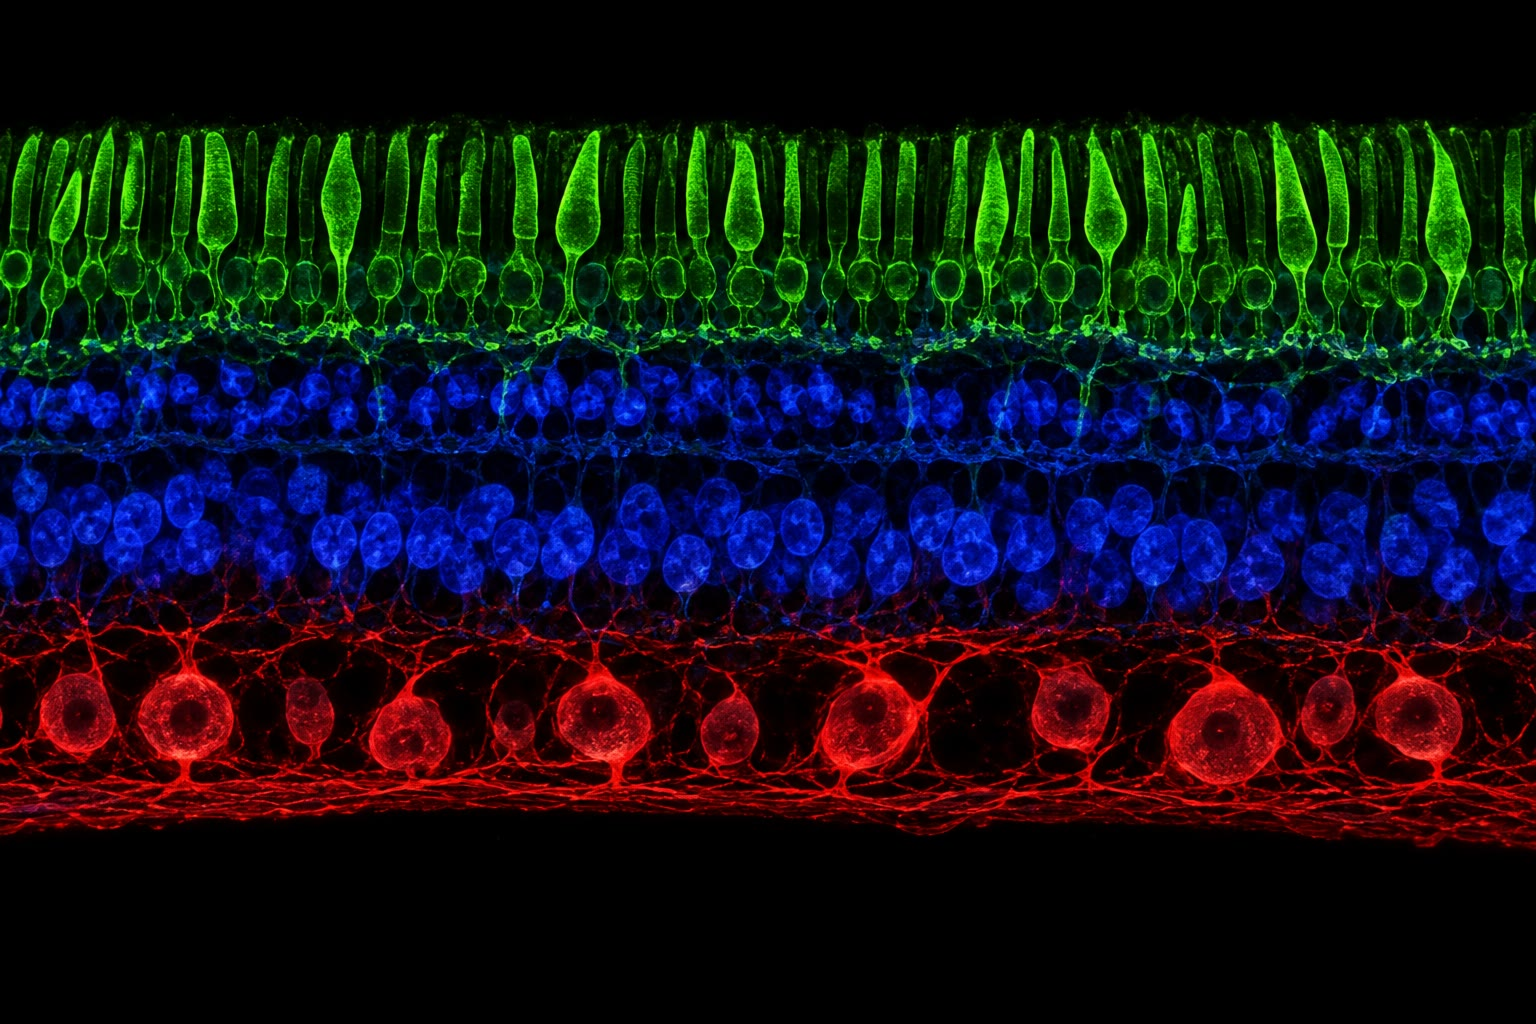
\includegraphics[width=0.46\linewidth]{images/book5/ai/b5-18-retina-section.jpg}\hspace{0.04\linewidth}
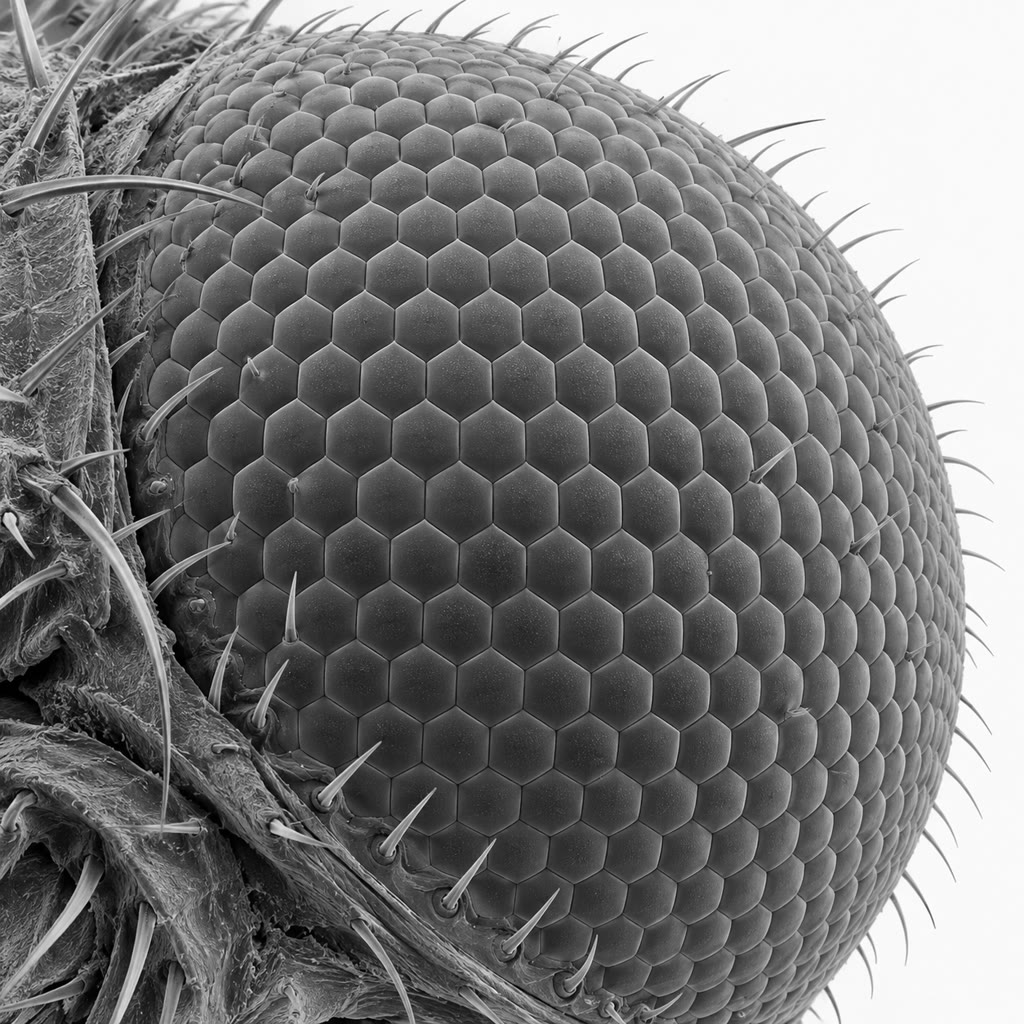
\includegraphics[width=0.36\linewidth]{images/book5/ai/b5-18-compound-eye.jpg}

{\small يسارًا: مقطع من \omterm{def:b3:sensory-systems:retina}{الشبكية}، والمستقبِلات الضوئية
(بالأخضر) في الخلف، ثم الخلايا ثنائية القطب والأفقية، ثم
الخلايا العقدية (بالأحمر) التي تغادر محاويرها إلى الدماغ.
ويمينًا: عين ذبابة مركّبة، مئات العدسات المنفصلة لكل منها
مستقبِلاتها --- وهو حل مختلف للمسألة نفسها.}
\end{omfigure}

\section{السمع والتوازن}

\begin{definition}[القوقعة]\label{def:b3:sensory-systems:cochlea}
\index{قوقعة}\index{غشاء قاعدي}\index{خريطة ترددية}\index{خلية شعرية}\index{أهداب صلبة}\index{وصلة قمية}\index{ديسيبل}
الصوت موجة ضغط؛ ومشكلة الأذن أن تكشف تغيّرات ضغط قدرها بضع
عشرات من الميكروباسكالات في الهواء وأن تفرزها بحسب التردد.
وتركّز طبلة الأذن وعُظيمات الأذن الوسطى الثلاثة القوةَ من
\qty{55}{mm^2} من الطبلة على \qty{3}{mm^2} من النافذة
البيضية، فترفع الضغط نحو عشرين ضعفًا --- وهي مطابقة الممانعة
بين الهواء وسائل الأذن الداخلية، ولولاها لانعكس معظم الصوت.
وداخل \emph{القوقعة}، وهي أنبوب ملفوف طوله \qty{35}{mm}،
تسير موجة الضغط على امتداد \emph{الغشاء القاعدي}، وهو ضيّق
صُلب عند القاعدة وعريض رخو عند القمة؛ وكل تردد يجعل الغشاء
يهتز أشد ما يهتز في موضع واحد --- فالترددات العالية قرب
القاعدة، والمنخفضة قرب القمة --- أي خريطة \emph{ترددية}
يقرؤها الدماغ طبقةً صوتية. وعلى الغشاء تجلس \emph{الخلايا
الشعرية}: \num{3500} خلية شعرية داخلية في صف واحد، كل واحدة
متوَّجة بحزمة من \emph{الأهداب الصلبة} موصولة قمةً بقمة
بواسطة \emph{وصلات قمية} دقيقة؛ وثني الحزمة نحو أطول أهدابها
يمطّط الوصلات ويفتح قنوات كاتيونية في غضون ميكروثوانٍ، بلا
أي رسول ثانٍ، فيتدفق البوتاسيوم داخلًا من اللمف الباطن،
الذي يعطي تركيبه غير المعتاد وكمونه $+\qty{80}{mV}$ قوة سوق
قدرها \qty{150}{mV}. والخلايا الشعرية الداخلية تشير إلى
العصب السمعي؛ وأما \num{12000} خلية شعرية خارجية، تسوقها
الحركة نفسها، فتنقبض وتستطيل مع الصوت بفضل البروتين الحركي
بريستين وتضخ طاقة راجعة إلى اهتزاز الغشاء --- أي مضخّم يحدّ
التنغيم مئة ضعف وهو ما يخفق في معظم حالات الصمم. وتُقاس
الشدة \emph{بالديسيبل}: $L = 10\log_{10}
(I/I_{0})$، حيث $I_{0} = \qty{1e-12}{W/m^2}$ عتبة السمع؛
وتعمل الأذن على مدى \qty{120}{dB}، أي تريليون ضعف في الشدة.
\end{definition}

\begin{omfigure}
\begin{tikzpicture}[every node/.style={font=\scriptsize}, >=stealth]
  % unrolled cochlea
  \begin{scope}
    \draw[thick, omDef, fill=omDef!10] (0,0.9) -- (7,1.4) -- (7,-1.4) -- (0,-0.9) -- cycle;
    \draw[very thick, omProp] (0,0.15) -- (7,-0.15); \draw[very thick, omProp] (0,-0.15) -- (7,0.15);
    \node[above] at (0.8,1.05) {القاعدة: ضيقة صلبة}; \node[above] at (6.2,1.5) {القمة: عريضة رخوة};
    \node[left, align=right] at (-0.1,0) {النافذة البيضية\\(من الرِّكاب)};
    \foreach \x/\f in {0.9/\qty{16}{kHz}, 2.3/\qty{4}{kHz}, 3.8/\qty{1}{kHz}, 5.4/\qty{250}{Hz}, 6.6/\qty{60}{Hz}} { \draw[omThm, thick] (\x,-0.55) -- (\x,0.55); \node[below, omThm] at (\x,-0.65) {\f}; }
    \node[below, align=center] at (3.5,-1.7) {الغشاء القاعدي (بالبرتقالي): كل تردد\\يهتز أشد ما يهتز في موضع واحد --- خريطة ترددية};
  \end{scope}
  % hair cell mechanism
  \begin{scope}[xshift=8.2cm, yshift=-0.6cm]
    \draw[thick, fill=omMeth!20] (0,0) rectangle (1.6,1.2); \node[below] at (0.8,-0.05) {خلية شعرية};
    \foreach \x/\h in {0.35/0.6, 0.65/0.85, 0.95/1.1, 1.25/1.35} \draw[very thick, omMeth!70!black] (\x,1.2) -- (\x,1.2+\h);
    \foreach \x/\h/\xx/\hh in {0.35/0.6/0.65/0.85, 0.65/0.85/0.95/1.1, 0.95/1.1/1.25/1.35} \draw[omThm, thick] (\x,1.2+\h) -- (\xx,1.2+\hh-0.1);
    \draw[->, thick] (1.9,2.3) -- (2.4,2.3) node[right, align=left, font=\tiny] {ثنيٌ نحو الأطول:\\تتمطط الوصلات القمية، وتُفتح\\القنوات في $\unit{\micro s}$؛ ويدخل K$^{+}$\\(بسوق \qty{150}{mV})};
    \node[above, align=center] at (0.8,2.7) {أهداب صلبة موصولة\\بوصلات قمية (بالأحمر)};
  \end{scope}
\end{tikzpicture}

{\small يسارًا: \omterm{def:b3:sensory-systems:cochlea}{القوقعة} مبسوطة --- \omterm{def:b3:sensory-systems:cochlea}{الغشاء القاعدي} يتدرج من
الصلب إلى الرخو، وكل تردد يبلغ ذروته في موضعه هو. ويمينًا:
حزمة شعرية، تفتح وصلاتها القمية قنوات التحويل ميكانيكيًا
حين تُثنى الحزمة.}
\end{omfigure}

\begin{proof}[شواهد]
فتح فون بيكيشي (في أربعينيات القرن العشرين) قواقع الجثث،
ونثر جسيمات فضة على \omterm{def:b3:sensory-systems:cochlea}{الغشاء القاعدي}، وراقب تحت ضوء ومّاض
كيف تقيم النغمات الصافية موجة سائرة تقع ذروتها أقرب إلى
القاعدة كلما ارتفعت النغمة --- وهي شفرة الموضع، التي نال
عليها جائزة نوبل عام 1961. ودفع هدسبث (في ثمانينيات القرن
العشرين) حزمة شعرية واحدة بليف زجاجي وسجّل التيار: فقد جرى
في غضون \qty{10}{\micro s} من الدفع، وهو أسرع بكثير من أي
شلال إنزيمي، وتناسب مع مقدار تحرك الحزمة نحو صفها الأطول،
وزال حين قُطعت الوصلات القمية بخالب كالسيوم. فالبوابة
ميكانيكية --- إذ تسحب الوصلة القناة فتفتحها --- ولذلك كان
السمع أسرع الحواس ولذلك يهدم محوّلَه الصوتُ العالي الذي
يقطع الوصلات.
\end{proof}

\begin{example}[أرقام الأذن]\label{ex:b3:sensory-systems:ear-numbers}
عند عتبة السمع يتحرك \omterm{def:b3:sensory-systems:cochlea}{الغشاء القاعدي} نحو \qty{0.1}{nm} وتكون
سعة الضغط \qty{20}{\micro Pa}، أي جزءًا من ملياري جزء من
الضغط الجوي؛ وعند \qty{120}{dB} يكون الضغط أكبر بمليون مرة
وحركة الغشاء عشرات النانومترات. والأذن الفتية تسمع من
\qty{20}{Hz} إلى \qty{20}{kHz} وتفصل نغمتين تتباعدان
\qty{0.3}{\%}، وقد حدّت الخلايا الشعرية الخارجية تمييز شفرة
الموضع. وتشتعل ألياف العصب السمعي البالغة \num{30000} على
خطى موجة الضغط حتى نحو \qty{4}{kHz} (القفل الطوري)، فتحمل
توقيتًا بدقة عشرات الميكروثواني، يحسب منها الدماغ اتجاه
الصوت من فرق الوصول إلى الأذنين --- وهو لا يتجاوز
\qty{10}{\micro s}. وتستعمل أعضاء التوازن الخلايا الشعرية
نفسها: ففي \emph{القنوات نصف الدائرية} يثنيها قصور السائل
الذاتي حين يستدير الرأس (تسارع زاوي)، وفي أعضاء الحصيات
تحمّلها طبقة من بلورات كربونات الكالسيوم بالجاذبية وبالتسارع
الخطي.
\end{example}

\begin{omfigure}
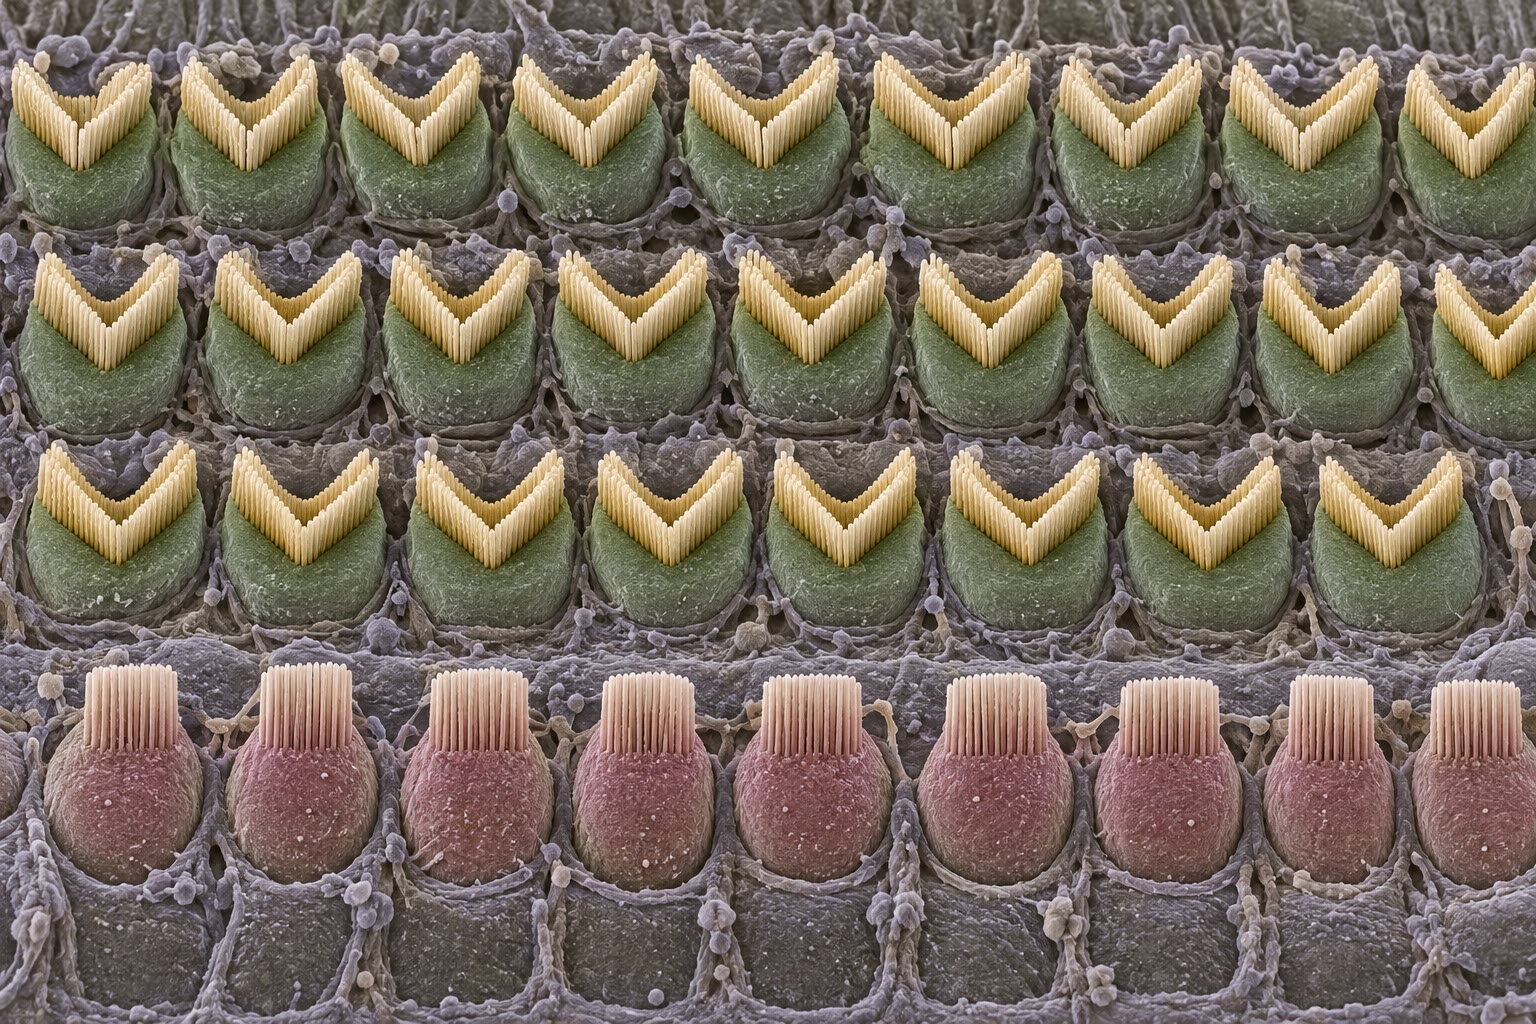
\includegraphics[width=0.54\linewidth]{images/book5/ai/b5-18-cochlea-hair-cells.jpg}

{\small عضو كورتي من فوق: ثلاثة صفوف من الخلايا الشعرية
الخارجية بحزم على شكل V، وصف واحد من الخلايا الشعرية
الداخلية. وتفتح الوصلات القمية في كل حزمة القنوات؛ فالخلايا
الخارجية تضخّم، والداخلية تخبر.}
\end{omfigure}

\section{الحواس الكيميائية}

\begin{definition}[الشم والذوق]\label{def:b3:sensory-systems:chemical}
\index{مستقبل شمّي}\index{شفرة توفيقية}\index{كبيبة}\index{ذوق}
يبدأ الشم في رقعة من الظهارة في أعلى الأنف، حيث يعبّر كل
واحد من نحو عشرة ملايين \emph{عصبون حسي شمّي} عن مورّثة
\emph{مستقبل شمّي} واحدة من نحو $400$ في الإنسان (و\num{1100}
في الفأر، وهي أكبر عائلة مورّثية في أي من الجينومين) ---
وهي مستقبلات مقترنة بالبروتين G ترتبط بجزيئات الرائحة في
جيب وتفتح، عبر AMP الحلقي، قناةً. ويربط كل مستقبل عدة
جزيئات رائحة ويربط كل جزيء رائحة عدة مستقبلات، فالرائحة
\emph{شفرة توفيقية}، أي نمط نشاط عبر أنماط المستقبِلات
البالغة $400$، وتغيّر كربون واحد في جزيء يغيّر النمط
والرائحة. وترسل العصبونات كلها المعبِّرة عن مستقبل واحد
محاويرها إلى \emph{الكبيبة} أو الكبيبتين نفسها في البصلة
الشمية، فتحوي البصلة خريطة تكون فيها كل رائحة نمطًا مكانيًا
من الكبيبات الفعالة، تقرؤه القشرة من غير مرور \omterm{def:b3:nervous-systems:plan}{بالمهاد}.
والذوق أبسط: خمسة أنماط، كل واحد \omterm{def:b3:sensory-systems:principles}{خط موسوم} من خلاياه
المستقبِلة --- الحلو والأومامي والمر عبر مستقبلات مقترنة
بالبروتين G (مستقبل واحد للحلو، وواحد للأومامي، ونحو خمسة
وعشرين للمر)، والملح عبر قناة صوديوم، والحامض عبر قناة
بروتونات --- وسائر ما نسميه النكهة هو الشم، يبلغ الأنف من
مؤخرة الفم.
\end{definition}

\begin{proof}[شواهد]
استدل باك وأكسل (1991) على أن مستقبلات الرائحة لا بد أن
تكون مستقبلات مقترنة بالبروتين G معبَّرًا عنها في الظهارة
الشمية وحدها، فوجدا بتفاعل PCR ببادئات منحلّة عائلة من مئات
هذه المورّثات، معبَّرًا عنها هناك ولا مكان سواه --- وهي
مستقبلات الشم، التي بقيت مجهولة قرنًا. وأظهر التهجين في
الموضع مستقبلًا واحدًا لكل عصبون وتقارب العصبونات المتشابهة
على كبيبات مفردة؛ وسجّل مالنيك وباك وزملاؤهما (1999) من
عصبونات مفردة وبيّنوا أن كل جزيء رائحة يفعّل عدة أنماط من
المستقبِلات وأن كل مستقبل يفعّله عدة جزيئات --- وتلك \omterm{def:b3:sensory-systems:chemical}{الشفرة
التوفيقية}. وطلب بوشديد وزملاؤه (2014) من مفحوصين تمييز
مخاليط فقدّروا أن الإنسان يقدر على تمييز أكثر من تريليون
رائحة، وهو أبعد بكثير من البضعة آلاف التي شاع الاعتقاد بها.
\end{proof}

\begin{proposition}[سعة الشفرة التوفيقية]\label{prop:b3:sensory-systems:combinatorial}
\index{شفرة توفيقية!السعة}
مع $R$ نمطًا من المستقبِلات كل واحد إما فعال وإما صامت، يمكن
تمثيل رائحة بأي من $2^{R}$ نمطًا؛ وعند $R = 400$ يكون ذلك
$10^{120}$، وحتى لو لم تُعتبر إلا الأنماط التي فيها $10$
أنماط فعالة بالضبط لكان هناك
$\binom{400}{10} \approx 3\times 10^{20}$. ولا يحدّ التمييزَ
الشفرةُ بل ضجيج المستقبِلات وقراءة الدماغ: فشفرة \omterm{def:b3:sensory-systems:principles}{الخط
الموسوم} بمستقبل واحد لكل رائحة تتيح $400$ رائحة، \omterm{def:b3:sensory-systems:chemical}{والشفرة
التوفيقية} تتيح أكثر مما يوجد من جزيئات تُشمّ. والثمن أن
مستقبلًا واحدًا لا يقول للدماغ إلا القليل بنفسه؛ فلا بد أن
يُقرأ النمط ككل، وهو ما تفعله خريطة الكبيبات والقشرة
الشمية.
\end{proposition}

\begin{omfigure}
\begin{tikzpicture}[every node/.style={font=\scriptsize}, >=stealth]
  % receptor rows, odorant columns
  \foreach \i/\lab in {1/المستقبل A, 2/المستقبل B, 3/المستقبل C, 4/المستقبل D, 5/المستقبل E} \node[left] at (-0.1,-0.7*\i) {\lab};
  \foreach \j/\lab in {1/هكسانول, 2/هبتانول, 3/أوكتانول, 4/ليمونين} \node[above, rotate=0] at (1.2*\j-0.6,-0.35) {\lab};
  \foreach \i/\j/\v in {1/1/100, 1/2/30, 2/1/60, 2/2/100, 2/3/50, 3/2/40, 3/3/100, 3/4/20, 4/3/70, 5/4/100, 1/4/30} \fill[omThm!\v] (1.2*\j-1.15,-0.7*\i-0.3) rectangle (1.2*\j-0.05,-0.7*\i+0.3);
  \foreach \i in {1,...,5} \foreach \j in {1,...,4} \draw[gray!50] (1.2*\j-1.15,-0.7*\i-0.3) rectangle (1.2*\j-0.05,-0.7*\i+0.3);
  \node[below, align=center] at (2.1,-4.1) {كل جزيء رائحة يفعّل مجموعة من المستقبِلات،\\وكل مستقبل مجموعة من جزيئات الرائحة:\\فالرائحة هي العمود};
  % glomerular map
  \begin{scope}[xshift=9.2cm, yshift=-2.2cm]
    \draw[thick, omDef!60, fill=omDef!8] (0,0) ellipse (2.6 and 1.7); \node[above] at (0,1.75) {البصلة الشمية: الكبيبات};
    \foreach \p in {(-1.8,0.6),(-1.0,1.0),(-0.2,0.7),(0.8,1.0),(1.7,0.5),(-1.6,-0.4),(-0.6,-0.6),(0.4,-0.3),(1.3,-0.7),(0.1,0.2)} \draw[omDef!70, fill=omDef!25] \p circle (0.25);
    \fill[omThm!80] (-1.0,1.0) circle (0.25); \fill[omThm!50] (0.4,-0.3) circle (0.25); \fill[omThm!80] (1.7,0.5) circle (0.25);
    \node[below, align=center] at (0,-1.8) {كل عصبونات نمط مستقبل واحد\\تتقارب على كبيبة واحدة: فالرائحة\\نمط مكاني (بالأحمر) تقرؤه القشرة};
  \end{scope}
\end{tikzpicture}

{\small \omterm{def:b3:sensory-systems:chemical}{الشفرة التوفيقية} للشم. يسارًا: مصفوفة مستقبِلات في
جزيئات رائحة، كل رائحة فيها نمط على امتداد عمود. ويمينًا:
النمط مبسوطًا على كبيبات البصلة.}
\end{omfigure}

\begin{omfigure}
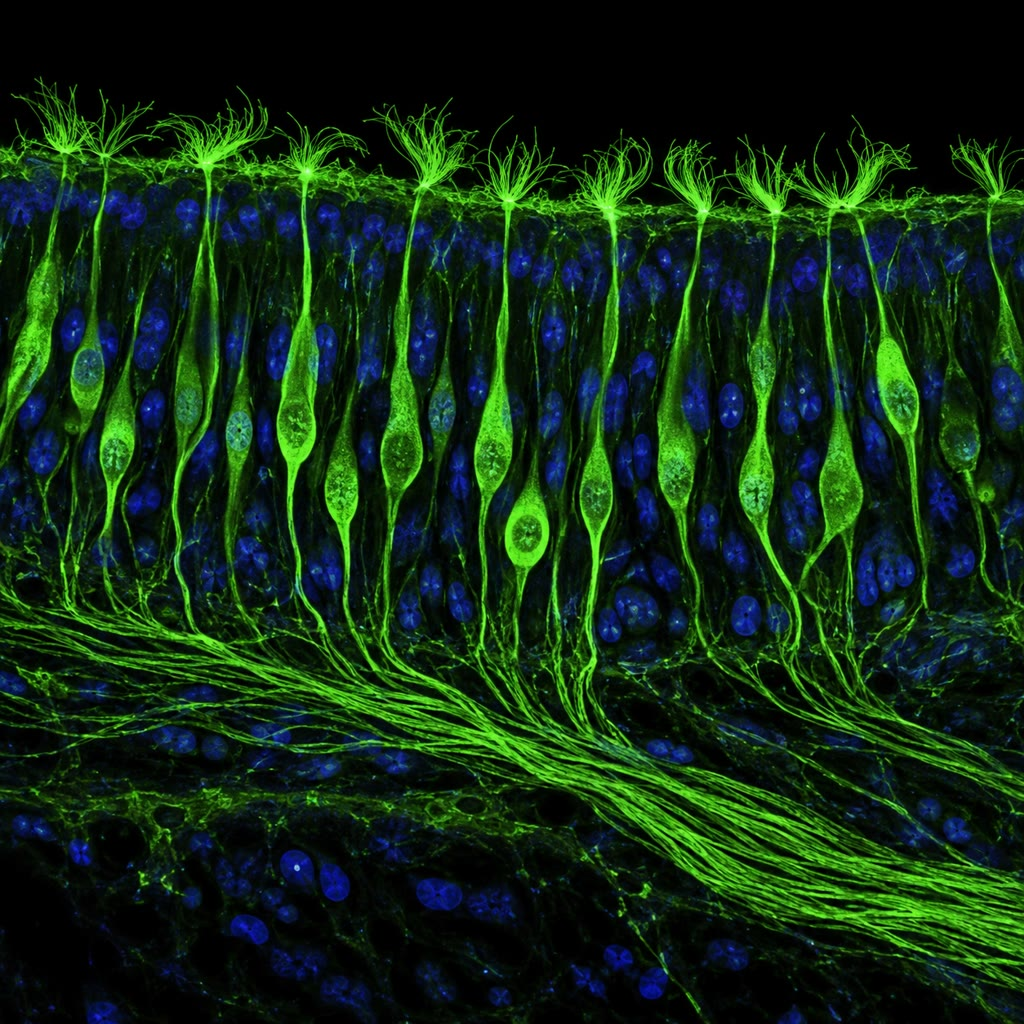
\includegraphics[width=0.40\linewidth]{images/book5/ai/b5-18-olfactory-epithelium.jpg}

{\small الظهارة الشمية: عصبونات حسية (بالأخضر) لها تغصنات
مهدّبة عند السطح، حيث ترتبط جزيئات الرائحة، ومحاوير تتحزم
أسفل نحو البصلة. ويعبّر كل عصبون عن مورّثة مستقبل واحدة من
الأربعمئة.}
\end{omfigure}

\section{اللمس، والحرارة، والألم، والحواس التي نفتقر إليها}

\begin{definition}[الحس الجسدي]\label{def:b3:sensory-systems:somato}
\index{مستقبل ميكانيكي}\index{قناة Piezo}\index{قناة TRP}\index{مستقبل الألم}\index{حس عميق}
يحوي الجلد عدة أنماط من \emph{المستقبِلات الميكانيكية}، كل
واحد محوار ينتهي في محفظته هو: خلايا ميركل للضغط الدقيق
والملمس (بطيئة التكيّف، حقولها صغيرة)، وجسيمات مايسنر للمس
الخفيف والانزلاق (سريعة التكيّف)، وجسيمات باتشيني عميقًا في
الجلد للاهتزاز (شديدة سرعة التكيّف، حقولها ضخمة)، ونهايات
روفيني للتمطط. والمحوّل في معظمها هو \emph{Piezo2}، وهي
قناة أيونية عملاقة ذات مروحة من الشفرات تنفتح حين يُمطَّط
الغشاء؛ ومن دونها يُفقد اللمس وحس وضع الجسم، والقناة نفسها
في الرئتين والمثانة تحس امتلاءهما. و\emph{الحرارة} تحسها
قنوات من عائلة TRP منغَّمة على مدايات مختلفة --- TRPV1،
تفتحها الحرارة فوق \qty{43}{\celsius} ويفتحها الكابسيسين،
ولذلك يكون الفلفل ``حارًّا''؛ وTRPM8، يفتحها البرد
والمنثول --- و\emph{الألم} تحسه نهايات عصبية حرة، هي
\emph{مستقبِلات الألم}، تستجيب للحرارة أو الضغط أو المواد
الكيميائية المؤذية (البروتونات، وATP، والبراديكينين)
ويخفض \omterm{def:b3:innate-immunity:inflammation}{الالتهاب} عتباتها (\cref{ch:b3:innate-immunity}).
و\emph{الحس العميق}، أي الإحساس بمواضع الأطراف، يأتي من
المغازل العضلية وأعضاء الأوتار في \cref{ch:b3:nervous-systems}
ومن Piezo2 في محافظ المفاصل. وتحدد كثافة المستقبِلات الحدة:
فنقطتان تتباعدان \qty{2}{mm} تُميَّزان على طرف الإصبع،
وتلزم \qty{40}{mm} على الظهر.
\end{definition}

\begin{method}[قياس حاسة]\label{met:b3:sensory-systems:psychophysics}
\index{فيزياء نفسية}\index{عتبة}\index{تمييز النقطتين}
لتوصيف قناة حسية: (1) جِد \emph{العتبة المطلقة} بعرض منبّهات
متدرجة الشدة مرات كثيرة ومطابقة نسبة المكشوف --- أي الشدة
التي تُكشف في نصف المرات --- كما فعل هِشت؛ (2) جِد
\emph{عتبة الفرق} عند شدات عدة وتحقق من \omterm{thm:b3:sensory-systems:weber}{قانون فيبر}؛ (3)
ارسم \emph{الحدة المكانية} بمنبّهين عند تباعدات مختلفة
(اختبار النقطتين على الجلد، ومحزّز على \omterm{def:b3:sensory-systems:retina}{الشبكية})؛ (4) ارسم
\emph{الحدة الزمنية} بالوميض أو بالنقرات (يندمج الوميض عند
نحو \qty{60}{Hz} في الإبصار النهاري)؛ (5) في حيوان، سجّل من
ألياف واردة مفردة أثناء تطبيق المنبّهات نفسها وطابق العتبات
العصبية بالسلوكية --- \omterm{met:b3:sensory-systems:psychophysics}{فالفيزياء النفسية} والفيزيولوجيا
ينبغي أن تتفقا، وحيث لا تتفقان يكون الفرق هو ما يضيفه
الدماغ.
\end{method}

\begin{remark}[حيوانات أخرى، وحواس أخرى]\label{rem:b3:sensory-systems:others}
لكل حاسة هنا صورة دفعها حيوان أبعد، وثمة حواس نفتقر إليها.
فالقروش والشفنينات تحس حقول الميكروفولت من نبض قلب فريسة
عبر قنوات مملوءة بهلام؛ والأسماك الكهربائية تقرأ تشوهات
حقلها هي لترى في الظلام. وأفاعي الحفرة تصوّر الفرائس الدافئة
بحفر حساسة للأشعة تحت الحمراء؛ والخفافيش والدلافين تحدد
الموضع بالصدى، فتوقّت أصداء نداءاتها بدقة بضعة ميكروثوانٍ
وتوجّه تردد النداء لتقفّي فراشة؛ والنحل يرى فوق البنفسجي
واستقطاب ضوء السماء ويهتدي به؛ والطيور المهاجرة والسلاحف
تحس حقل الأرض المغناطيسي بآلية لا تزال موضع جدل. وأنف الكلب
فيه من العصبونات المستقبِلة أربعون ضعف ما في أنفنا وثلث
دماغه لقراءتها؛ والبومة تسمع فأرًا تحت الثلج. والمبادئ لا
تتغير --- محوّل، \omterm{def:b3:sensory-systems:principles}{وخط موسوم}، وشفرة، وضغط، وخريطة --- والتنوع
هو ما صنعه التطور بها.
\end{remark}

\section{تمارين}

\begin{exercise}[$\star$]\label{exo:b3:sensory-systems:1}
اشرح كيف يعرف الدماغ هل جاء قطار الشوكات من العين أم من
الأذن، مع أن الشوكات متطابقة.
\end{exercise}

\begin{exercise}[$\star$]\label{exo:b3:sensory-systems:2}
لماذا يفرط الضوء استقطاب مستقبِل ضوئي، وما تيار الظلام؟
\end{exercise}

\begin{exercise}[$\star$]\label{exo:b3:sensory-systems:3}
الهمس \qty{20}{dB}، والمحادثة \qty{60}{dB}، وحفلة الروك
\qty{110}{dB}. احسب شدة كل منها بوحدة W/m$^{2}$ والنسبة بين
الأعلى والأخفت.
\end{exercise}

\begin{exercise}[$\star$]\label{exo:b3:sensory-systems:4}
اذكر أنماط \omterm{def:b3:sensory-systems:chemical}{الذوق} الخمسة وأنماط مستقبِلاتها، واشرح لماذا
يحجب الزكام ``\omterm{def:b3:sensory-systems:chemical}{ذوق}'' الطعام.
\end{exercise}

\begin{exercise}[$\star\star$]\label{exo:b3:sensory-systems:5}
كسر فيبر للوزن $0.02$. فانطلاقًا من وزن \qty{100}{g}، كم
خطوة ملحوظة بالكاد تقع بينه وبين \qty{10}{kg}؟ استعمل صيغة
فِشنر وتحقق بعدّ خطوات بعامل $1.02$.
\end{exercise}

\begin{exercise}[$\star\star$]\label{exo:b3:sensory-systems:6}
استنادًا إلى \cref{thm:b3:sensory-systems:hecht}، احسب $P_{\text{see}}$ عند
$a = 2$ و$6$ و$12$ فوتونًا ممتصًّا وبعتبة $n = 6$. وعند أي
$a$ تُرى الومضة في نصف المرات؟ وإذا امتُصّ \qty{10}{\%} من
الفوتونات عند القرنية، فكم يجب أن توصل الومضة؟
\end{exercise}

\begin{exercise}[$\star\star$]\label{exo:b3:sensory-systems:7}
تركّز الأذن الوسطى القوة من \qty{55}{mm^2} على \qty{3}{mm^2}
برافعة قدرها $1.3$. فبأي عامل يرتفع الضغط، وكم ذلك
\omterm{def:b3:sensory-systems:cochlea}{بالديسيبل}؟ ولماذا تكون أذن شخص التحمت عُظيماته الوسطى
(التصلب الأذني) أبلد بعشرات الديسيبلات؟
\end{exercise}

\begin{exercise}[$\star\star$]\label{exo:b3:sensory-systems:8}
اشرح لماذا يظهر تيار التحويل في \omterm{def:b3:sensory-systems:cochlea}{خلية شعرية} في غضون
ميكروثوانٍ بينما يستغرق تيار المستقبِل الضوئي عشرات
الميلي ثانية، وماذا تكسب كل حاسة من تصميمها.
\end{exercise}

\begin{exercise}[$\star\star$]\label{exo:b3:sensory-systems:9}
للفأر \num{1100} نمط مستقبِل وللإنسان $400$. فإذا فعّلت
رائحة نحو \qty{5}{\%} من الأنماط، كم نمطًا بهذا الحجم
بالضبط متاح لكل منهما (استعمل $\binom{R}{k}$ عند $k = 0.05R$،
وتقريب ستيرلنغ $\ln\binom{R}{k} \approx R\,H(k/R)$ حيث
$H(p) = -p\ln p - (1-p)\ln(1-p)$)؟
\end{exercise}

\begin{exercise}[$\star\star\star$]\label{exo:b3:sensory-systems:10}
تمثلن \omterm{def:b3:sensory-systems:retina}{العصيّة} رودوبسينًا عفويًا مرة كل \qty{40}{s} في
الظلام. ففي رقعة من $500$ \omterm{def:b3:sensory-systems:retina}{عصيّة} تُرصد في نافذة \qty{0.1}{s}،
ما وسطي عدد الأحداث العفوية، وما احتمال وقوع ستة أو أكثر
مصادفةً؟ واشرح لماذا يضع الدماغ العتبة عند نحو ستة لا عند
واحد.
\end{exercise}

\begin{exercise}[$\star\star\star$]\label{exo:b3:sensory-systems:11}
يقفل العصب السمعي شوكاته على طور الصوت حتى \qty{4}{kHz}،
باهتزاز قدره نحو \qty{20}{\micro s}. والصوت يسير بسرعة
\qty{340}{m/s} والأذنان متباعدتان \qty{20}{cm}. فما أكبر
تأخير بين الأذنين، وأي تمييز زاوي يعطيه تمييز قدره
\qty{10}{\micro s} قرب الخط الأوسط، ولماذا تخدم شفرة الموضع
لا التوقيت فوق \qty{4}{kHz}؟
\end{exercise}

\begin{exercise}[$\star\star\star$]\label{exo:b3:sensory-systems:12}
يجعل \omterm{def:b3:sensory-systems:principles}{التثبيط الجانبي} حقلًا رماديًا منتظمًا بجوار حقل داكن
يبدو أفتح عند الحد. نمذج صفًا من المستقبِلات يهيّج كل واحد
منها ضوؤه هو $I_{i}$ ويثبّطه كسر $w$ من ضوء كل جار، أي
$r_{i} = I_{i} - w(I_{i-1} + I_{i+1})$، واحسب الاستجابة عبر
قفزة من $I = 1$ إلى $I = 2$ عند $w = 0.2$. فماذا تكسب
\omterm{def:b3:sensory-systems:retina}{الشبكية} وماذا تخسر بذلك؟
\end{exercise}

\section{مسألة: شمعة تُرى من بعيد}

\begin{problem}[{مسألة نهاية الأسبوع --- فوتونات شمعة تُعدّ
داخلةً إلى عين بعيدة، وكشف الومضة يُحسب من إحصاء بواسون
ومضخّم العصيّة، وديسيبلات حفلة تُحوَّل إلى حركة طبلة أذن
وتيار خلية شعرية، وشفرة أنف تُحصى، وتُختم بالمسافة التي
تُرى عندها الشمعة، وبالضغط عند طبلة الأذن، وبالأنماط التي
يقدر أنف على تكوينها}]
\label{pb:b3:sensory-systems:1}
المعطيات: تصدر شمعة نحو \qty{0.01}{W} من الضوء المرئي، عند
\qty{550}{nm} (وطاقة الفوتون $3.6\times 10^{-19}$ جول).
وحدقة متكيّفة على الظلام قطرها \qty{7}{mm}؛ ويمتص
\omterm{def:b3:sensory-systems:retina}{الرودوبسين} \qty{10}{\%} من الفوتونات الداخلة إلى العين؛
وتكامل العين على \qty{0.1}{s}؛ والعتبة $6$ فوتونات ممتصّة.
وكل فوتون ممتصّ يغلق $200$ قناة ويخفض تيار الظلام
\qty{1}{pA} مدة \qty{0.2}{s}؛ وتيار الظلام في \omterm{def:b3:sensory-systems:retina}{العصيّة}
\qty{30}{pA}. والصوت: $I_{0} =
\qty{1e-12}{W/m^2}$؛ ومساحة طبلة الأذن \qty{55}{mm^2}؛ وحزمة
شعرية ارتفاعها \qty{5}{\micro m} تنحرف عند العتبة
\qty{0.3}{nm}. والشم: $R = 400$ مستقبل؛ وتيار التحويل في
\omterm{def:b3:sensory-systems:cochlea}{الخلية الشعرية} \qty{100}{pA} عند التشبع.

\medskip
\noindent\textbf{الجزء الأول --- الفوتونات.}
\begin{enumerate}
  \item كم فوتونًا في الثانية تصدر الشمعة؟
  \item على بعد $d$ تنتشر الفوتونات على كرة مساحتها
        $4\pi d^{2}$. فكم يدخل منها الحدقة في الثانية عند
        \qty{1}{km}؟ وعند \qty{10}{km}؟
  \item كم يُمتصّ في نافذة تكامل واحدة عند كل مسافة؟ وهل
        تُرى الشمعة (العتبة $6$)؟
  \item جِد المسافة التي يساوي عندها وسطي العدد الممتصّ في
        نافذة $6$. وبإحصاء بواسون، أي نسبة من النوافذ تتجاوز
        العتبة هناك؟
  \item عند مسافة السؤال 4، ما احتمال ألا تحوي نافذة
        \qty{0.1}{s} بعينها أي فوتون البتة؟ ولماذا يبدو نجم
        خافت وامضًا؟
  \item تحت بدر تمتص العصيّات نفسها $10^{4}$ فوتون في النافذة
        من السماء. اشرح لماذا تصير الشمعة عند \qty{10}{km}
        غير مرئية عندئذ مع أنها توصل الفوتونات نفسها.
\end{enumerate}

\medskip
\noindent\textbf{الجزء الثاني --- مضخّم \omterm{def:b3:sensory-systems:retina}{العصيّة}.}
\begin{enumerate}[resume]
  \item فوتون واحد يغلق $200$ قناة ويخفض التيار \qty{1}{pA}.
        فأي تيار تحمل قناة واحدة، وكم كاتيونًا في الثانية
        ذلك ($e = \qty{1.6e-19}{C}$)؟
  \item أي نسبة من تيار الظلام يزيل فوتون واحد؟ وكم فوتونًا
        متزامنًا يطفئ \omterm{def:b3:sensory-systems:retina}{العصيّة} إطفاءً تامًا (التشبع)؟
  \item تدوم الاستجابة \qty{0.2}{s}. فكم كاتيونًا يمنع فوتون
        واحد من الدخول؟ وما الكسب في الشحنة لكل فوتون؟
  \item في ضوء النهار يبلغ \omterm{def:b3:sensory-systems:retina}{العصيّة} $10^{5}$ فوتون في
        الثانية. فماذا يحدث لها، ولماذا تكون المخاريط، التي
        تتكيّف وتتشبع أقل، مستقبِلات النهار؟
  \item تحتاج المخاريط إلى نحو $100$ فوتون لتشير. اشرح، من
        حيث المقايضة بين الحساسية والسرعة، لماذا تستجيب
        المخاريط في \qty{20}{ms} والعصيّات في \qty{200}{ms}.
  \item يتمثلن \omterm{def:b3:sensory-systems:retina}{الرودوبسين} عفويًا مرة كل \qty{40}{s}. فعلى
        $10^{8}$ \omterm{def:b3:sensory-systems:retina}{عصيّة} في العين، كم فوتونًا كاذبًا في الثانية
        تولّد \omterm{def:b3:sensory-systems:retina}{الشبكية}، ولماذا لا يُعمي ذلك العين المظلمة
        بالضجيج؟ (فكّر في العتبة وفي \omterm{def:b3:sensory-systems:principles}{الحقل الاستقبالي}.)
\end{enumerate}

\medskip
\noindent\textbf{الجزء الثالث --- الديسيبلات.}
\begin{enumerate}[resume]
  \item حفلة عند \qty{110}{dB}: الشدة بوحدة W/m$^{2}$ والقدرة
        الساقطة على طبلة أذن واحدة.
  \item كم طاقة صوتية تتلقى طبلة الأذن في حفلة مدتها
        ساعتان؟ وقارن ذلك بطاقة قطرة مطر ساقطة
        (\qty{1e-4}{J}).
  \item عتبة السمع عند \qty{0}{dB}: القدرة على طبلة الأذن
        والطاقة في كل \qty{10}{ms} --- وقارن ذلك بطاقة فوتون
        مرئي واحد.
  \item تنحرف الحزمة الشعرية \qty{0.3}{nm} عند العتبة على
        ارتفاع \qty{5}{\micro m}. فأي زاوية تلك، بالدرجات؟
        وقارن الانحراف بقطر ذرة هدروجين (\qty{0.1}{nm}).
  \item التعرض المطوَّل فوق \qty{85}{dB} يؤذي الخلايا
        الشعرية، والخلايا الشعرية لا تتجدد في الثدييات.
        فساعتان عند \qty{110}{dB} توصلان من الطاقة قدر كم
        ساعة عند \qty{85}{dB}؟
  \item مدى السمع \qty{120}{dB}. فكم خطوة ملحوظة بالكاد من
        الجهارة ذلك، إذا كان كسر فيبر للشدة نحو $0.25$
        (\omterm{def:b3:sensory-systems:cochlea}{ديسيبل} واحد)؟
\end{enumerate}

\medskip
\noindent\textbf{الجزء الرابع --- شفرة الشم.}
\begin{enumerate}[resume]
  \item مع $400$ مستقبل كل واحد إما فعال وإما مطفأ، كم نمطًا؟
        اكتب الجواب أسًّا للعشرة.
  \item إذا فعّلت رائحة عادةً $20$ مستقبلًا، كم نمطًا متمايزًا
        من هذا القبيل ($\binom{400}{20}$، استعمل ستيرلنغ أو
        اللوغاريتمات)؟
  \item يتشارك جزيئا رائحة $15$ من مستقبِلاتهما البالغة
        $20$. اقترح مقياسًا لبُعدهما في الشفرة واشرح لماذا
        تتشابه رائحتاهما.
  \item يميّز الإنسان نحو تريليون رائحة. فأي نسبة من أنماط
        السؤال 20 ذلك، وما الذي يحد العدد دون سعة الشفرة
        بكثير؟
  \item فأر له \num{1100} مستقبل: كم نمطًا من $20$ أكثر من
        الإنسان، أسًّا للعشرة؟
  \item طفرة تحذف مورّثة مستقبل واحدة. تنبأ بأثرها في القدرة
        على الشم عمومًا وفي إدراك جزيء رائحة واحد يرتبط بذلك
        المستقبل ارتباطًا قويًا (فقد الشم النوعي).
  \item لخّص: المسافة التي تُرى عندها الشمعة (السؤال~4)،
        والطاقة الصوتية على طبلة الأذن عند العتبة في
        \qty{10}{ms} (السؤال~15)، وعدد أنماط العشرين مستقبلًا
        التي يقدر أنف بشري على تكوينها (السؤال~20).
\end{enumerate}
\end{problem}
